\documentclass{beamer}
\usetheme[numbering=fullbar]{focus}
\setbeamertemplate{mini frames}{}
\usepackage{subfig}
\usepackage{graphicx}
\usepackage[export]{adjustbox}
\usepackage[version=4]{mhchem}
\usepackage{fix-cm}

\title{Lung Development \& \\ Pattern Formation}
\subtitle{Math 638 Final Presentation}
\author{Geneva Porter}
\titlegraphic{
\includegraphics[scale=.3]{Images/fingerprint.png}}
\institute{San Diego State University\\ Applied Mathematics}
\date{\today}

\begin{document}
\AtBeginSection{}

    \begin{frame}
        \maketitle
    \end{frame}

    \begin{frame}{Overview}
        \tableofcontents
    \end{frame}
    
    \section[Introduction]{Introduction, Background, and Research Motivation}
        \subsection{The Developing Lung}
        
            \begin{frame}{\insertsubsectionhead}
            
                \begin{columns}
                    \column{0.55\textwidth}
                        \begin{figure}
                            \centering
                            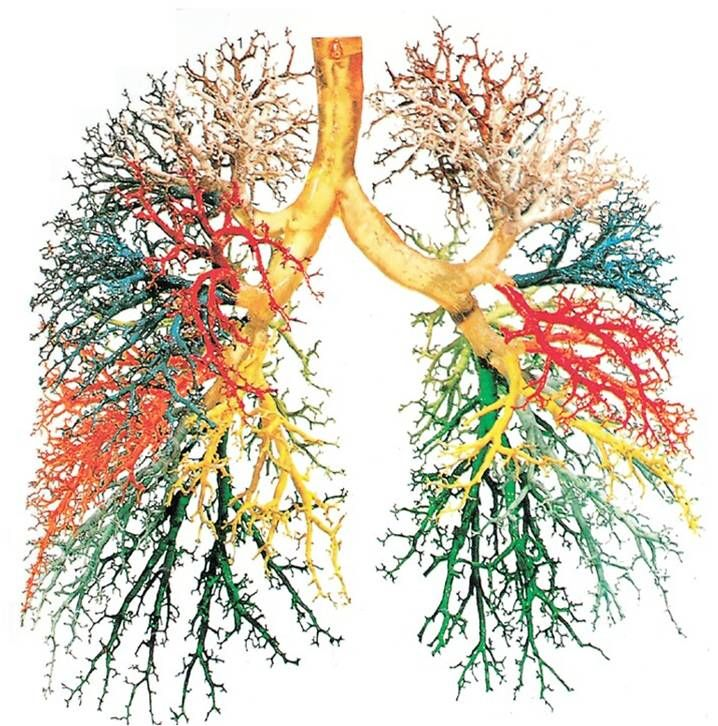
\includegraphics[width=5cm, frame]{Images/v2lung01.jpg}
                            \caption{Human bronchial tree of adult male, color coded.}
                        \end{figure}
                    \column{0.45\textwidth}
                    This research examines the pseudoglandular stage of vertebrate lung development and the role of two gene proteins in branching morphogenesis: Fibroblast Growth Factor 10 \textbf{FGF10} and Sonic Hedgehog gene \textbf{SHH}. These proteins form a feedback loop.$^\cite{Prince2018}$
                \end{columns}
            
            \end{frame}
        
            \begin{frame}{\insertsubsectionhead}
                \begin{figure}
                    \centering
                    
                    \subfloat[Branching at the pseudoglandular stage]{\reflectbox{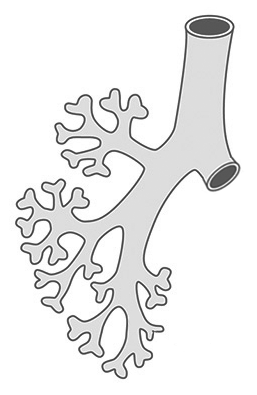
\includegraphics[width=3cm, height=4cm,frame]{Images/lungs2.png}}}\qquad %\pause
                    \subfloat[Gene proteins diffuse from lung surface]{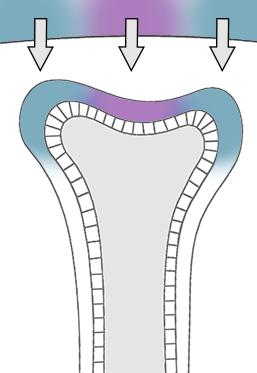
\includegraphics[width=3cm, height=4cm,frame]{Images/lungs3.png}}\qquad %\pause
                    \subfloat[Feedback loop between FGF10 and SHH genes]{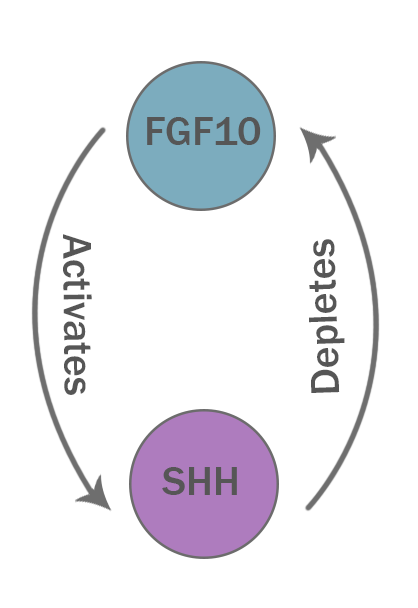
\includegraphics[width=3cm, height=4cm,frame]{Images/genes1.png}}
                    
                \end{figure}
            
            \end{frame}
            
            \begin{frame}{\insertsubsectionhead}
            
                \begin{columns}
                    \column{0.55\textwidth}
                        \textbf{Applications to lung regeneration and disease research:} \\
                         \vspace{5mm}
                        Congenital Diaphragmatic Hernias (CDH) causes hypoplastic lung development in the fetus. There is currently no treatment to encourage continued branching growth postpartum.$^\cite{Pearse2018}$
                    \column{0.45\textwidth}
                        \begin{figure}
                            \centering
                            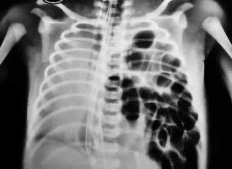
\includegraphics[width=5cm, frame]{Images/v2lung02.jpg}
                            \caption{Left-sided CDH in infant}
                        \end{figure}
                \end{columns}
            
            
            
            \end{frame}
            
        \subsection{Analysis Approach}
        
            \begin{frame}{\insertsubsectionhead}
            
                \begin{center}
                    {\Large Reaction-Diffusion Equations}\\
                    $\frac{\partial u}{\partial t}=D_u\Delta u+f(u,v)$\\
                    $\frac{\partial v}{\partial t}=D_v\Delta v+g(u,v)$\\
                    \vfill
                    
                    %\pause
                    {\Huge \textbf{+}} \\
                    \vfill
                    
                    {\Large Turing Instability Regions}\\
                    The system is \textbf{stable} \textit{without} the diffusion terms. \\
                    The system is \textbf{unstable} \textit{with} the diffusion terms. \\
                    \vfill
                    
                    %\pause
                    {\Huge \textbf{=}} \\
                    \vfill
                    
                    {\Large Pattern Formation Model} \\
                    The deviation from homogeneity yielding a domain \\with nonuniform concentrations of morphogens$^\cite{Turing1952}$
                
                \end{center}
            
            \end{frame}
            
            \begin{frame}{\insertsubsectionhead}
                
                \vfill
                
                Schnakenberg$^\cite{Schnakenberg1979}$ considered a simple kinetic model for a reaction-diffusion system that emphasized the activator- depletion relationship between two morphogens: 
                
                \begin{Large}
                $$ \ce{X <=>[k_1][k_2] F} ~~~~~~~~~~ \ce{2F + S ->[k_3] 3F} ~~~~~~~~~~ \ce{Y ->[k_4] S} $$
                \end{Large}
                
                $F(r,\phi,\theta,t)$ is the activator concentration for the FGF10 gene.
                $S(r,\phi,\theta,t)$ is for depletion substrate, or the SHH gene.
                \vfill
                
                And $X$ and $Y$ are precursor substrate concentrations.
                \vfill
            
            \end{frame}
            
            \begin{frame}{\insertsubsectionhead}
            
                \vfill
                
                This analysis will replace the diffusion term in the classic reaction-diffusion model with the surface Laplacian $\Delta_\Gamma$, defined:
                \vfill
                
                \begin{equation*}
                    \label{Laplace-Beltrami}
                    \Delta_\Gamma u = \nabla_\Gamma\cdot\nabla_\Gamma u ~~~~~ \text{with} ~~~~~ \nabla_\Gamma u = \nabla u-(\nabla u\cdot\vec{n})\vec{n}
                \end{equation*}
                \vfill
                 The resulting hybrid model of a reaction-diffusion system on the surface of a sphere is given by:
                
                
                \begin{Large}
                \begin{equation*}
                    \begin{aligned}
                    \dot{F} & = D_F\Delta_\Gamma F + k_1 - k_2F + k_3F^2S \\
                    & \\
                    \dot{S} & = D_S\Delta_\Gamma S + k_4 - k_3F^2S \\
                    \end{aligned}
                \end{equation*}
                \end{Large}
            
            \end{frame}
            
            \begin{frame}{\insertsubsectionhead}
                
                
                \begin{equation*}
                    \begin{aligned}
                    \dot{F} ~~~
                     &=~~~ \overbrace{D_F\Delta_\Gamma F}^\text{diffusion} ~~~
                    +\overbrace{k_1}^\text{rate constant} 
                    ~~~- \overbrace{k_2F}^\text{degradation} + 
                    ~~\overbrace{k_3F^2S}^\text{autocatalysis}&  \\
                    \dot{S} ~~~ 
                     &=~~~ \underbrace{D_S\Delta_\Gamma S}_\text{diffusion} 
                    ~~~+\underbrace{k_4}_\text{rate constant} 
                    ~~~-\underbrace{k_3F^2S}_\text{autocatalysis}&  \\
                    \end{aligned}
                \end{equation*}
                
                \begin{description}
                    \item[~~~~~~~~~~Diffusion] Net movement of substrates
                    \item[Rate Constant] Precursor substrate production of FGF10 and SHH
                    \item[~~~Degradation] FGF10 is catalyzed to a precursor substrate
                    \item[~Autocatalysis] FGF10 uses SHH for self-production
                \end{description}
                
            
            \end{frame}
        
    \section[Turing Regions]{Turing Instability Regions}
    
        \subsection{Stability Without Diffusion}
        
            \begin{frame}{\insertsubsectionhead}
                
                Using scaling substitutions, we get:
                
                $$\alpha = \frac{k_1}{k_2}\sqrt{\frac{k_3}{k_2}} ~~~~~ \beta = \frac{k_4}{k_2}\sqrt{\frac{k_3}{k_2}} ~~~~~ \delta = \frac{D_S}{D_F} ~~~~~ \text{and} ~~~~~ \gamma = k_2 $$ 
                
                \vfill
                
                \begin{equation*}
                    \begin{aligned}
                        & \dot{F} = \Delta_\Gamma F + 
                        \gamma\left(\alpha - F + F^2S\right) ~~=  \Delta_\Gamma F + \gamma ~ f(F,S)\\
                        & \dot{S} = \delta\Delta_\Gamma S + 
                        \gamma\left(\beta - F^2S\right)~~~~~~~ = \delta\Delta_\Gamma S + \gamma ~ s(F,S)\\
                    \end{aligned}
                \end{equation*}
                
                \vfill
                
                Eliminating the diffusion terms, the fixed points are:
                
                \vfill
                
                $$(F^*,S^*)=\left(\alpha+\beta,\frac{\beta}{(\alpha+\beta)^2}\right)$$
                
                \vfill
            
            \end{frame}
            
            \begin{frame}{\insertsubsectionhead}
            
                To determine stability a perturbation is made:
        
                \begin{equation*}
                    \begin{aligned}
                    F = F^*+\varepsilon~\tilde{F} ~~~~~\longrightarrow~~~~~& \dot{F} = \varepsilon~\tilde{F}_t = \gamma~f(F^*+\varepsilon~\tilde{F})\\
                    S = S^*+\varepsilon~\tilde{S} ~~~~~\longrightarrow~~~~~& \dot{S} = \varepsilon~\tilde{S}_t = \gamma~s(S^*+\varepsilon~\tilde{S})
                    \end{aligned}
                \end{equation*}
                
                With some substitutions and a Taylor expansion:
                
                \begin{equation*}
                    \left(\begin{aligned}
                    \tilde{F}_t \\
                    \tilde{S}_t
                \end{aligned}\right)
                =
                \gamma\left(\begin{aligned}
                    f_F(F^*,S^*) ~~~~~& f_S(F^*,S^*)\\
                    s_F(F^*,S^*) ~~~~~& s_S(F^*,S^*) \\
                \end{aligned}\right)
                \cdot
                \left(\begin{aligned}
                    \tilde{F} \\
                    \tilde{S}
                \end{aligned}\right)
                + \mathcal{O}(\varepsilon^2)
                \end{equation*}
                
                Or more simply:
                \Huge$$\dot{W}=\gamma~J^*W$$
                
                \vfill
                
            \end{frame}
            
            \begin{frame}{\insertsubsectionhead}
            
                \vfill
                
                The Jacobian is evaluated to be:
                
                \vfill
                
                $$ J^* =  \left(
                \begin{aligned}
                    -1+\frac{2\beta}{\alpha+\beta} ~~&~~~~ (\alpha+\beta)^2 \\
                    -\frac{2\beta}{\alpha+\beta} ~~~~&~~ -(\alpha+\beta)^2
                \end{aligned} \right)$$
                
                \vfill
                
                Yielding the eigenvalues:
                
                \vfill
                
                \begin{equation*}
                    \lambda = \frac{\gamma}{2}\left( \frac{\beta-\alpha}{(\alpha+\beta)}-(\alpha+\beta)^2\pm\sqrt{\left(\frac{\alpha-\beta}{\alpha+\beta}+(\alpha+\beta)^2\right)^2-4(\alpha+\beta)^2}\right)
                \end{equation*} 
                
                \vfill
            
            \end{frame}
        
            \begin{frame}{\insertsubsectionhead}
            
                \center{Stable parameters: ~~~ $ \beta-\alpha < (\alpha+\beta)^3 $}
                \vspace{-5mm}
                \begin{figure}[H]
                    \centering
                    \subfloat[Stability region for $\alpha$ and $\beta$ values]{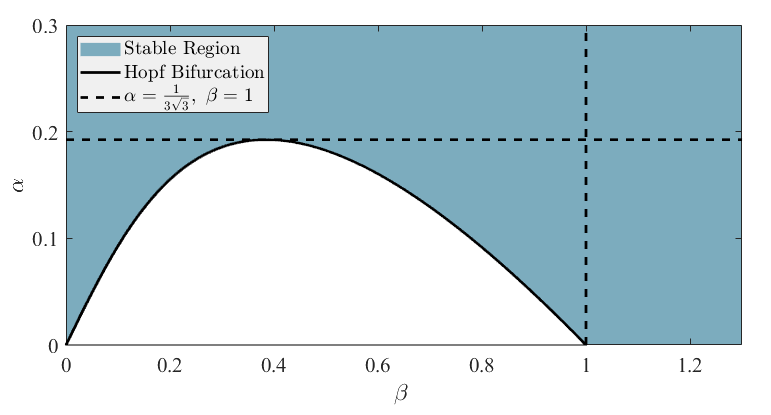
\includegraphics[width = 9cm]{Images/stability_region2.png}}
                \end{figure}

            \end{frame}
            
        \subsection{The Eigenvalue Problem}
        
            \begin{frame}{\insertsubsectionhead}
            
                \begin{center}
                
                Without diffusion, there was $\dot{W}=\gamma~J^*W$. With diffusion:
                $$\dot{W}=D\Delta_\Gamma W+\gamma~J^*W$$
                
                To turn this into a linear system:
                $$ \dot{W}=\lambda W ~~~~~\text{and}~~~~~ \Delta_\Gamma W = -k^2W $$
                
                This yields  the eigenfunctions for $W$:
                $$e^{\lambda t},~~~P_n^m(\cos{\phi}),~~~\text{and}~~~e^{im\theta} ~~~~~\text{with} ~~~m=0,1,2,...~~~\text{and}~~~n\geq m$$
                
                Leaving the linear system:
                \Large
                $$ \lambda W = -Dk^2 W+\gamma J^*W$$
                
                \end{center}
            
            \end{frame}
        
        \subsection{Instability with Diffusion}
        
            \begin{frame}{\insertsubsectionhead}
            
            The parameter constraints for \textbf{instability} with diffusion are:
            
            $$ \det(  - Dk^2 + \gamma~J^*-\lambda I ) = 0 ~~~\text{and}~~~ \exists ~\text{Re}[\lambda(k^2)] > 0 $$
            
            Which gives the characteristic equation:
            
            $$\lambda^2 - \lambda[\gamma~(f_F+s_S)-k^2(1+\delta)] + h(k^2)=0$$
            $$ \text{Where } ~ h(k^2) = \delta k^4-\gamma~(\delta f_F + s_S)k^2 + \gamma\det(J^*) $$
            
            For instability: 
            $$\text{Re}[\lambda(k^2)]>0 ~~~~~\longrightarrow ~~~~~ \gamma~(\delta f_F+s_S)k^2 > \delta k^4+\gamma\det(J^*)$$
            
            \end{frame}
            
            \begin{frame}{\insertsubsectionhead}
            
                \vspace{-5cm}
                {\fontsize{90}{100}\selectfont 
                $$\delta > 1 $$}
                
                \vspace{1cm}
                \centering
                Therefore, SHH must diffuse faster than FGF10
                
            \end{frame}
            
    \section[Results]{Results and Patterns}
    
        \subsection{Analytical Solution}
    
            \begin{frame}{\insertsubsectionhead}
            
                \vfill
                
                Here is the analytic solution to the \textbf{eigenvalue} problem.
                \vfill
                {\Large
                $$W(\phi,\theta,t)=\sum_{m=0}^\infty \sum_{n=m}^\infty A_{mn}\cdot e^{\lambda t}\cdot Y_n^m(\phi,\theta)$$}
                
                \vfill \centering
                With 
                \vfill
                {\Large
                $$A_{mn}=\frac{\int_0^\pi\int_{-\pi}^\pi \left(_{S^*}^{F^*}\right)Y_n^m(\phi,\theta)\sin{\phi}d\theta d\phi}{\int_0^\pi\int_{-\pi}^\pi [Y_n^m(\phi,\theta)]^2\sin{\phi}d\theta d\phi}$$}
                
                \vfill
                
                
            \end{frame}
        
        \subsection{Surface Diffusion Patterns}
        
            \begin{frame}{\insertsubsectionhead}
            
                \begin{figure}
                    \centering
                    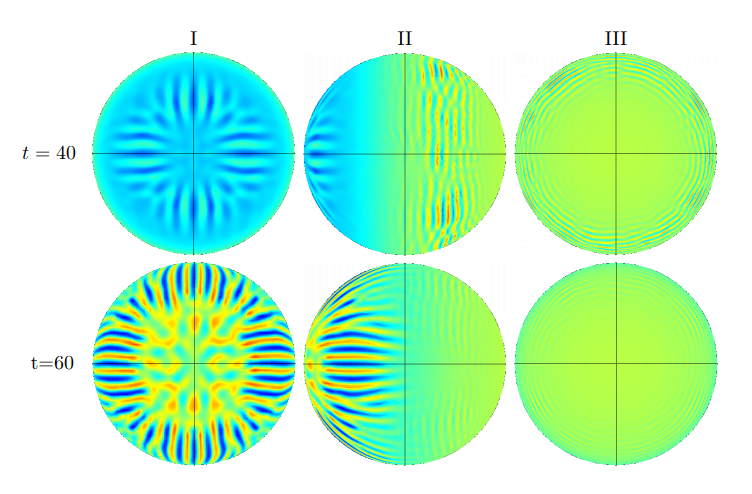
\includegraphics[width=8cm, frame]{Images/sol01.png}
                    \caption{R=100, $\alpha=0.1$, $\beta=0.9$, $\delta=10$, $\gamma=4$^\cite{Krause2018}}
                \end{figure}
            
            \end{frame}
            
            \begin{frame}{\insertsubsectionhead}
            
                \begin{figure}
                    \centering
                    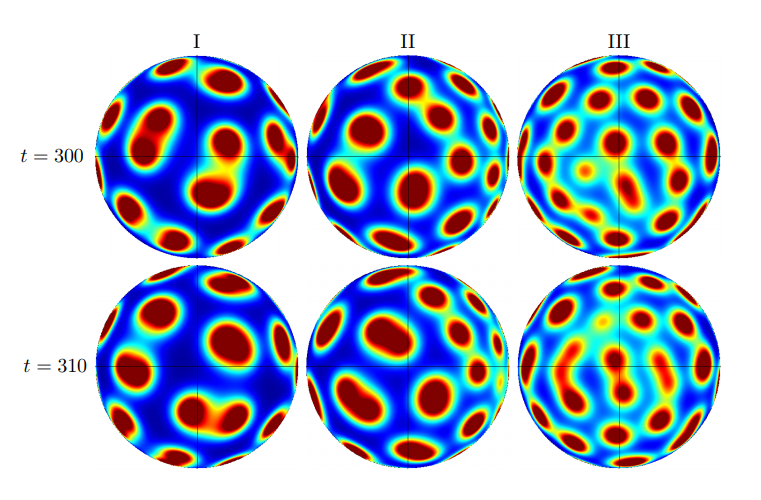
\includegraphics[width=8cm, frame]{Images/sol02.png}
                    \caption{r=20, $\alpha=0.1$, $\beta=0.9$, $\delta=20$, $\gamma=0.5$^\cite{Krause2018}}
                \end{figure}
            
            \end{frame}
            
            \begin{frame}{\insertsubsectionhead}
            
                \begin{figure}
                    \centering
                    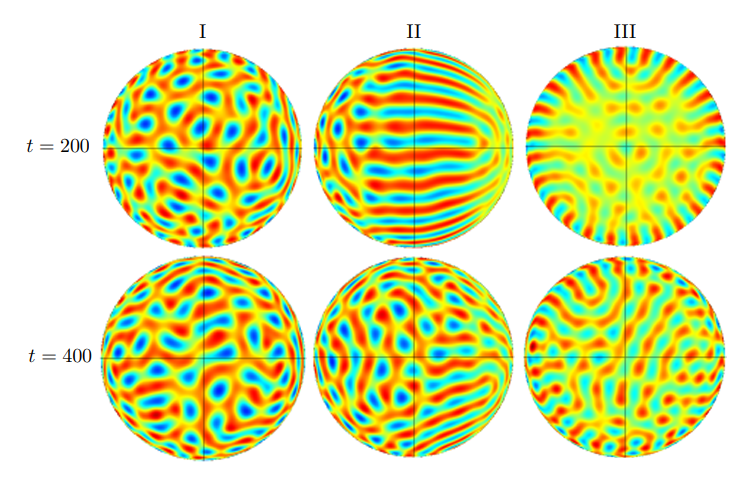
\includegraphics[width=8cm, frame]{Images/sol03.png}
                    \caption{r=40, $\alpha=0.01$, $\beta=1.2$, $\delta=10$, $\gamma=0.1$^\cite{Krause2018}}
                \end{figure}
                
            \end{frame}
        
    \section[Future Work]{Next Steps and Future Work}
        
            \begin{frame}{Next Steps and Future Work}
            
                \vfill
            
                \begin{columns}
                
                \column{0.5\textwidth}
                    {\Large Thesis Goals:}
                    \vspace{5mm}
                    \begin{itemize}
                    \item Examine model on the mesh of a human lung
                    \item Use surface finite element method for numerical solutions
                    \item Solve on growing domain
                    \end{itemize}
                    
                \column{0.5\textwidth}
                    \begin{figure}
                            \centering
                            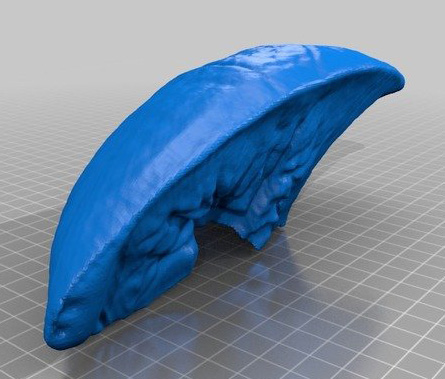
\includegraphics[width = 5cm, frame]{Images/v2lung03.jpg}
                            \caption{3D model of left lung}
                        \end{figure}
                    
                
                \end{columns}
                \vfill
            
            \end{frame}
            
            \appendix
            
            \begin{frame}{References}
                \nocite{*}
                \bibliography{demo_bibliography}
                \bibliographystyle{ieeetr}
            \end{frame}
    
            \begin{frame}[focus]
                Thank You!
            \end{frame}
    
\begin{frame}{Frame Title}
    \Large
        \begin{align*}
        &\Huge{\dot{F} = \Delta_\Gamma F + \gamma (\alpha - F + F^2S)} \\
        \\
        &\dot{S} = \delta\Delta_\Gamma S + \gamma (\beta - F^2S)\\
    \end{align*}
    
\end{frame}
    

\end{document}
